\documentclass[format=sigconf]{acmart}
\usepackage{minted}
\usepackage{xcolor}
\usepackage{xspace}
\usepackage[utf8]{inputenc}
\usepackage[T1]{fontenc}
\usepackage{amsmath}
\usepackage{amssymb}
\usepackage{stmaryrd}
\usepackage{graphicx}
\usepackage{varioref}   %
\usepackage{hyperref}
\usepackage[nameinlink,capitalize]{cleveref}
\usepackage{tocloft}
\usepackage{amsthm} % example env
\usepackage{enumitem} % description env
\usepackage{tikz}
\usepackage{pgfplots}
\usepackage[normalem]{ulem}

\newcommand\asterism{\medskip\noindent\textcolor{black!65}{\small\centerline{$\phantom{x}_{*\,\,\,*}^{\,\,\,*}$}}\smallskip}
\newcommand\intvl[1]{\llbracket#1\rrbracket}

\usemintedstyle{xcode}
\newminted{cl}{autogobble,breaklines,escapeinside=||,fontsize=\footnotesize}

\newcommand\code[2][\small]{\sloppy\texttt{#1#2}}
\newcommand\mcode[2][\small]{\text{\code[#1]{#2}}}
\newcommand\footcode[1]{\code[\scriptsize]{#1}}

\theoremstyle{definition}
\newtheorem{example}{Example}

\usetikzlibrary{positioning,shapes,shadows}


\bibliographystyle{alpha}

\acmConference[ELS'19]{the 19th European Lisp Symposium}{April 01--02 2018}{Genova, Italy}
\acmISBN{978-2-9557474-2-1}
\acmDOI{}

\title{Implementing Baker's SUBTYPEP decision procedure}

\author{Léo Valais}
\email{lvalais@lrde.epita.fr}
\orcid{0000-0000-0000-0000}

\author{Jim E. Newton}
\email{jnewton@lrde.epita.fr}
\orcid{0000-0002-1595-8655}

\author{Didier Verna}
\email{didier@lrde.epita.fr}
\orcid{0000-0002-6315-052X}

\affiliation{%
  \institution{EPITA/LRDE}
  \streetaddress{14-16 rue Voltaire}
  \postcode{94270}
  \city{Le Kremlin-Bic{\^e}tre}
  \country{France}
}

\begin{CCSXML}
<ccs2012>
<concept>
<concept_id>10003752.10003790.10011740</concept_id>
<concept_desc>Theory of computation~Type theory</concept_desc>
<concept_significance>500</concept_significance>
</concept>
<concept>
<concept_id>10003752.10003809.10011254.10011257</concept_id>
<concept_desc>Theory of computation~Divide and conquer</concept_desc>
<concept_significance>300</concept_significance>
</concept>
<concept>
<concept_id>10003752.10003809.10010031.10010032</concept_id>
<concept_desc>Theory of computation~Pattern matching</concept_desc>
<concept_significance>100</concept_significance>
</concept>
</ccs2012>
\end{CCSXML}

\ccsdesc[500]{Theory of computation~Type theory}
\ccsdesc[300]{Theory of computation~Divide and conquer}
\ccsdesc[100]{Theory of computation~Pattern matching}


\newcommand\sbcl{\textsc{Sbcl}}
\newcommand\then{$\rightarrow$}

\begin{document}


% \toappear{}
\begin{abstract}
  We present here our partial implementation of Baker's decision procedure for
  \code{subtypep}. In his article ``A Decision Procedure for Common Lisp's
  \code{SUBTYPEP} Predicate'', he claims to provide implementation guidelines to
  obtain a \code{subtypep} more accurate and as efficient as the average
  implementation. However he did not provide any serious implementation and his
  description is sometimes obscure. In this paper we present our implementation
  of part of his procedure, only supporting primitive types, \textsc{Clos}
  classes, \code{member}, range and logical type specifiers.
  We explain in our words our understanding of his procedure, with much more
  detail and examples than in Baker's article. We therefore clarify many parts
  of his description and fill in some of its gaps or omissions.
  We also argue in favor and against some of his choices and present our
  alternative solutions. We further provide some proofs that might
  be missing in his article and some early efficiency results. We have not
  released any code yet but we plan to open source it as soon as it is
  presentable.
\end{abstract}

\maketitle

\section{Introduction}
The Common Lisp standard \cite{bib:ansi.94.cl} provides the predicate function
\code{subtypep} for
introspecting the sub-typing relationship. Every invocation \code{(subtypep A B)}
either returns the values \code{(t t)} when \code{A} is a subtype of \code{B},
\code{(nil t)} when not, or \code{(nil nil)} meaning the predicate could not
(or failed to) answer the question. The latter can happen when the type
specifier \code{(satisfies P)} (representing the type $\{x \mid
\mathtt{P(x)}\}$ for some predicate and total function\footnote{A function
  defined over its entire definition domain.} \code{P}) is involved. For example,
given two arbitrary predicates \code{F} and \code{G}, there is no way
\code{subtypep} can answer the question \code{(subtypep '(satisfies F)
  '(satisfies G))}.

However, some implementations abuse the permission to return \code{(nil nil)}.
For example, in \sbcl{} 1.4.10 (the implementation we are currently focusing our
efforts on), {\small\code{(satisfies 'boolean 'keyword)}} returns
\code{(nil nil)}, thus violating the standard\footnote{The Common Lisp standard
  requires that no invocation of \footcode{subtypep} involving only primitive types
  return \footcode{(nil nil)}.}. The definition of the \code{keyword} type is
responsible for this failure: as shown in Listing \ref{lst:keyword}, it
involves a \code{satisfies} type specifier\footnote{%
  C.f. bug \#1533685 in \sbcl{} bug tracker.
}.

Another kind of problem for which \code{subtypep}'s accuracy matters is the
optimization of the \code{typecase} construct as shown in \cite{newton.18.phd}
and \cite{newton.18.els}. The aim is to remove redundant checks in the construct
and the approach is to use binary decision diagrams. However, to build such a
structure, \code{subtypep} is repeatedly used. The unreliability of the
predicate leads here to many lost BDD reductions and therefore to the
generation of sub-optimal code.

Our implementation is still in active development, currently targets
\sbcl{} and focuses almost entirely on result accuracy. It supports
\emph{primitive} types, \emph{user-defined} types (\code{deftype}, classes and structures),
\emph{\code{member} (and \code{eql})} type specifiers and \emph{ranges} (e.g.,
\code{(integer * 12)}). We present our strategy for implementing each one
of these while discussing how and why we decided or not to diverge from Baker's
\cite{baker1992}
approach---or potentially filling some gaps or unclear bits.
No optimization work has been done yet and the implementation still has
bugs and diverse issues, but we have found some encouraging results about
accuracy and even about efficiency.

\begin{listing}
  \begin{clcode}
(sb!xc:deftype keyword ()
  '(and symbol (satisfies keywordp)))
  \end{clcode}
  \caption{The \code{keyword} type definition in \sbcl}
  \label{lst:keyword}
\end{listing}


\section{The Common Lisp type system}
\label{sec:cltypes}
\subsection{Type specifiers}
Common Lisp types are not manipulated directly as they are in other languages
such as C++. Instead, the type to be
manipulated is \emph{described} using a \emph{type specifier}.
The type specifier Domain-Specific Language (DSL) allows programmers to
describe types by writing S-expressions which obey some rules described in the
Common Lisp standard \cite{bib:ansi.94.cl} and roughly summarized in
table~\ref{tab:ts}\footnote{More type specifiers exist. We do not describe them
  here either because we do not support them yet or because Baker's procedure
  ignores them as well.}.

A subtlety about type specifiers is that \emph{different ones} can
represent the \textit{same} type (e.g., \code{integer}, \code{(integer * *)} and
\code{(or fixnum bignum)} all describe the same type). This means that
\emph{symbolic computation does not suffice} to answer the sub-typing question.
Note that one could write a predicate, say \code{type=}, to determine whether
two type specifiers in fact describe the same type using two calls of
\code{subtypep}.

It is possible to define \emph{parametric aliases} using the \code{deftype}
construct. It is then possible to refer to a whole type specifier using its
alias. Listing \ref{lst:deftype} shows an example of parametric
\code{deftype}.

\begin{listing}
\begin{clcode}
(deftype except (x)
  `(not (eql ,x)))
\end{clcode}
\caption{The \code{deftype} construct}
\label{lst:deftype}
\end{listing}

\begin{table*}
  \centering
  \newcommand\var[1]{{\color{gray}$#1$}}
  \newcommand\pat[1]{\texttt{\small #1}}
  \begin{tabular}{rl|c}
    \hline
    Type specifier pattern & Description & Example \\
    \hline
    \pat{nil} & The null type $\emptyset$ & --- \\
    \pat{\var{u}}
            & A \code{symbol}-designated type & \code{character} \\
    \pat{(eql \var{e})}
            & The singleton type $\{e\}$ & \code{(eql 12)} \\
    \pat{(member \var{e_1} $\cdots$ \var{e_n})}
            & The type $\{e_1, \cdots, e_n\}$ & \code{(member t nil)} \\
    \pat{(not \var{u})}
            & The complement type $\overline{u}$ & \code{(not null)} \\
    \pat{(or \var{u_1} $\cdots$ \var{u_n})}
            & The union type $u_1 \cup \cdots \cup u_n$ & \code{(or integer float)} \\
    \pat{(and \var{u_1} $\cdots$ \var{u_n})}
            & The intersection type $u_1 \cap \cdots \cap u_n$ & \code{(and symbol (not keyword))} \\
    \pat{(\var{u} \var{X} \var{Y})}
            & The range $\{n \in u \mid X \leq n \leq Y\}$ & \code{(integer 1 6)} \\
    \pat{(\var{u} (\var{X}) \var{Y})}
            & The range $\{n \in u \mid X < n \leq Y\}$ & \code{(integer (0) 6)} \\
    \pat{(\var{u} * (\var{Y}))}
            & The range $\{n \in u \mid n < Y\}$ & \code{(integer * (43))} \\
    \pat{(array \var{u} \var{n})}
            & $n$-dimensional array of elements of type $u$ & \code{(array integer 1)} \\
    \pat{(array * (\var{d_1} $\cdots$ \var{d_n}))}
            & Array with $d_i$ elements in its $i$-th dimension & \code{(array * (3 3))} \\
    \pat{(array \var{u} (* * *))}
            & 3-dimensional $u$ array & \code{(array symbol (* * *))} \\
    \pat{(satisfies \var{p})} & The type $\{x \mid p(x)\}$ & \code{(satisfies oddp)} \\
    \hline
  \end{tabular}
  \caption{Brief summary of the type specifier DSL features}
  \label{tab:ts}
\end{table*}

\subsection{Vocabulary}
\begin{description}[leftmargin=8em,style=nextline]
  \item[type] A set of elements. For any type $u$: $u \equiv \{x \mid x\!:\!u\}$
  \item[canonical t.s.] A type specifier without aliases.
  \item[primitive type] A standardized type
    (\cite{bib:ansi.94.cl.type-specifiers}) that is not necessarily implemented
    as a class.
  \item[symbolic form] A type specifier whose type is \code{symbol}.
  \item[compound form] A type specifier whose type is \code{list}.
  \item[logical form] A compound form whose car is \code{or}, \code{and} or \code{not}.
  \item[kingdom] In Baker's terminology, a ``type kingdom'' designates the types
    that can be described using \emph{only one kind of type specifier}.
    \code{nil} (the empty type) belongs to every type kingdom.
  \item[interval] A mathematical interval that may not be a valid type specifier.
  \item[type $\approx$ t.s.] When unambiguous, we write type specifiers where a
    mathematical type is expected and to use a type variable, say $U$, as a
    placeholder inside Lisp code for \emph{a type specifier describing} $U$.
  % \item[$U \subseteq U'$] The type $U$ is a non-strict subtype of $U'$.
  %   We always have \code{(subtypep $U$ $U'$)}.
\end{description}

In this article we focus on two particular type kingdoms:
\begin{itemize}
\item the \emph{literal type kingdom}, represented using only
  symbolic, \code{member} and logical type specifiers, and,
\item the \emph{range type kingdom}, represented only using
  range and logical type specifiers
\end{itemize}

There are other type kingdoms that Baker mentions in his article, such as the
\emph{array} type kingdom, represented using only \code{array} and logical type
specifiers. Note that a type can belong to several kingdoms, as multiple type
specifiers can describe it. For example, \code{integer} belongs to literal
\emph{and} range kingdoms as the type specifiers \code{integer} (symbolic) and
\code{(integer * *)} (range) both describe it. In Section \ref{sec:pre}, we
describe how to guarantee that a given type is only described by one kind of
type specifier, hence restricting it to \emph{one} kingdom.

\section{Procedure's mechanisms overview}
\label{sec:flow}
Figure \ref{fig:flow} shows the internals of our implementation. Every step will
be detailed in the following sections. There are three \emph{major stages}:

\begin{enumerate}
\item \emph{The pre-processing} --- Both type specifiers are processed in order to
  simplify further calculations: the aliases are expanded, and each occurrence
  of numeric types are converted to their equivalent range type specifier.
  Finally, as explained thereafter, the procedure splits into several
  sub-procedures, one for each type kingdom, because their internal
  type representation differ. In order to achieve that, the type specifiers must
  also be split into equivalent subtype specifiers restricted to each concerned
  kingdom.
  This stage is detailed in Section \ref{sec:pre}.
\item \emph{Expert sub-procedures} --- Once split, each subtype specifier is
  redirected to the appropriate expert sub-procedure. The job of such a procedure is to
  \emph{prove}, in its own kingdom, the assertion ``$A$ is a subtype of $B$'' to
  be \emph{wrong}.
  Our procedures currently only support literal and range type specifiers---an
  expert sub-procedure has been implemented only for these two kingdoms. This
  stage is detailed in Section \ref{sec:exp}.
\item \emph{Result conjunction} --- Eventually, all expert sub-procedures
  return (a Boolean) and the results are accumulated using conjunction.
  (In practice, as soon as one expert procedure returns false, \code{subtypep}
  returns.)
\end{enumerate}

\begin{figure}
  \centering
  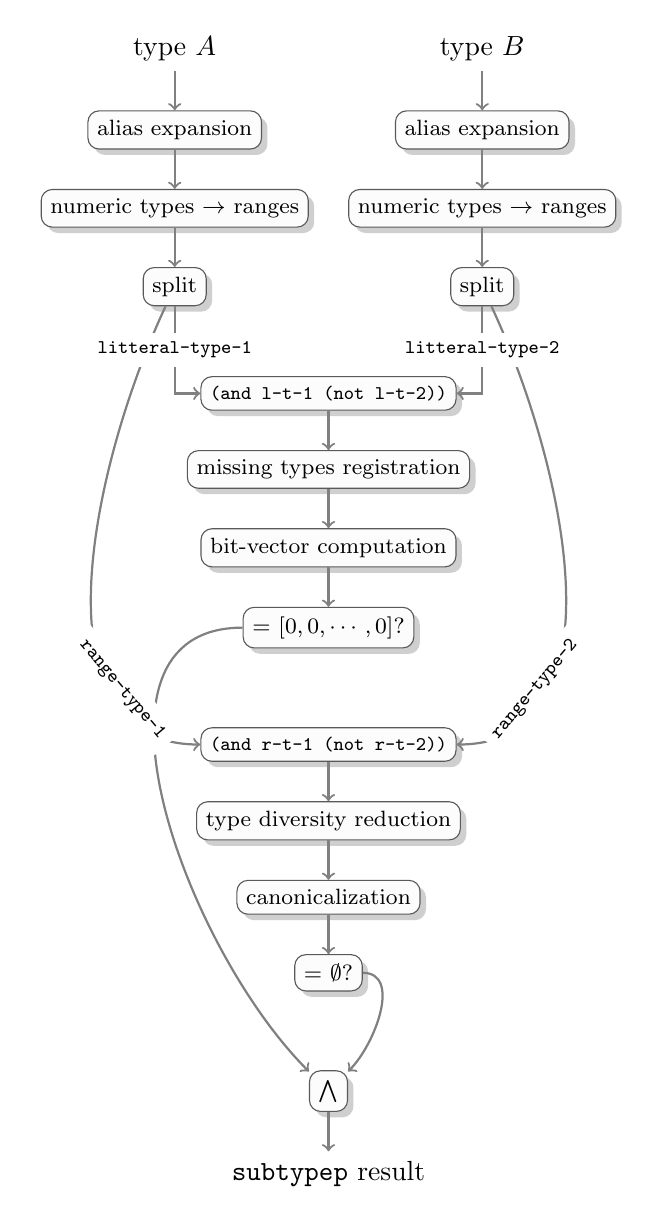
\begin{tikzpicture}[node distance=5mm,
  action/.style={rectangle,rounded corners,fill=white,drop shadow=gray!75,draw=black!65,fill=gray!2,font=\footnotesize},
  andnot/.style={action,font=\scriptsize\tt},
  arrow/.style={->,thick,gray},
  label/.style={fill=white,text=black,font=\tt\scriptsize},
  inout/.style={}
  ]
  \def\longest{numeric types \then{} ranges}

  \node[action] (largest1) {\longest};
  \node[action,right=of largest1] (largest2) {\longest};
  \node[action,above=of largest1] (typexpand1) {alias expansion};
  \node[action,above=of largest2] (typexpand2) {alias expansion};
  \node[action,below=of largest1] (split1) {split};
  \node[action,below=of largest2] (split2) {split};
  \node[inout,above=of typexpand1] (a) {type $A$};
  \node[inout,above=of typexpand2] (b) {type $B$};
  \draw[arrow,opacity=0] (largest1) -- (largest2) node[midway,opacity=0] (middle) {};

  \node[andnot,below=2 of middle] (andnotL) {(and l-t-1 (not l-t-2))};
  \node[action,below=of andnotL] (reg) {missing types registration};
  \node[action,below=of reg] (bv) {bit-vector computation};
  \node[action,below=of bv] (nullbv) {= $[0,0,\cdots,0]$?};

  \node[andnot,below=1 of nullbv] (andnotR) {(and r-t-1 (not r-t-2))};
  \node[action,below=of andnotR] (red) {type diversity reduction};
  \node[action,below=of red] (canon) {canonicalization};
  \node[action,below=of canon] (nullin) {= $\emptyset$?};

  \node[action,below=1 of nullin] (conj) {$\bigwedge$};
  \node[inout,below=of conj] (res) {\texttt{subtypep} result};


  \draw[arrow] (a) to (typexpand1);
  \draw[arrow] (b) to (typexpand2);
  \draw[arrow] (typexpand1) to (largest1);
  \draw[arrow] (typexpand2) to (largest2);
  \draw[arrow] (largest1) to (split1);
  \draw[arrow] (largest2) to (split2);

  \draw[arrow] (split1) to [out=245,in=180] (andnotR);
  \draw[arrow] (split2) to [out=295,in=0] (andnotR);
  % near start = pos=0.1
  \draw[arrow] (split1) |- (andnotL) node[label,near start] (lt1) {litteral-type-1};
  \draw[arrow] (split2) |- (andnotL) node[label,near start] (lt2) {litteral-type-2};

  \draw[arrow] (andnotL) to (reg);
  \draw[arrow] (reg) to (bv);
  \draw[arrow] (bv) to (nullbv);
  \draw[arrow] (andnotR) to (red);
  \draw[arrow] (red) to (canon);
  \draw[arrow] (canon) to (nullin);

  \draw[arrow] (nullbv) to [out=180,in=135] (conj);
  \draw[arrow] (nullin) to [out=0,in=45] (conj);
  \draw[arrow] (conj) to (res);

  % tricky labels to place
  \node[label,left=.41 of andnotR,rotate=-50] (rt1) {range-type-1};
  \node[label,right=.41 of andnotR,rotate=50] (rt2) {range-type-2};
\end{tikzpicture}

  \caption{Internal flowchart of \code{(subtypep $A$ $B$)}}
  \label{fig:flow}
\end{figure}

\section{Pre-processing}
\label{sec:pre}
\subsection{Alias expansion}
The very first step is to ensure that the type specifier is in its
\emph{canonical form}, that is, having all its aliases expanded. This is done by
the \code{expand} function. For example, considering the type created in
Listing \ref{lst:deftype}, \code{(expand '(except 12))} should return \code{(not
  (eql 12))}.

Unlike macro expansion, \code{deftype} expansion is not standardized in Common
Lisp. Thus a solution must be found for each Common Lisp implementation
independently. As our efforts are currently focused on \sbcl{}, we discuss
how we implement the \code{expand} function for that compiler.

\sbcl's \code{subtypep} heavily relies on the function
\code{sb-kernel:specifier-type}, which does type expansion. It also does
type simplification---turning \code{(and integer string)} into
\code{nil}---which could have saved us some work. We hoped we could simplify
that function to make it compatible with Baker's algorithm while keeping the
\code{deftype} expansion and the range canonicalization work. However we found,
thanks to \cite{newton.18.phd} tools, that the function is responsible for most
of the work of \code{subtypep}, as shown in Figure \ref{fig:specifiertype}
\footnote{The \footcode{cached-subtypep-caching-call} is just a memoizing wrapper
  around \sbcl's \footcode{subtypep} which is a bit more efficient than the raw
  implementation}.
Considering the lack of efficiency of that function and the fact that it would
not be trivial to simplify it to only keep the interesting bits, we decided to
stick to another, more cost-effective solution.

The function \code{sb-ext:typexpand} takes a type specifier and tries to expand
it (not recursively). It either returns the expansion result, or the input type
specifier if it is not expandable. \code{(sb-ext:typexpand 'integer)} returns
\code{integer} since it is not a \code{deftype} alias whereas
\code{(sb-ext:typexpand '(except 12))} returns \code{(not (eql 12))}.
To expand a whole type specifier, it just needs to walk through it, applying
\code{sb-ext:typexpand} on each list or atom manually. One subtlety though is
that the result of an expansion may itself be an alias to
expand\footnote{%
  Fortunately, \footcode{sb-ext:typexpand} also returns a Boolean indicating
  whether or not an expansion happened.%
}. For example, let's say that we have
\code{(deftype my-type () '(except 0.0))}, then the result of
\code{(sb-ext:typexpand 'my-type)} is \code{(except 0.0)}, which is of course an
alias to expand again.

\begin{figure}
  \centering
  \newcommand\profgraph[1]{\includegraphics[scale=.40]{#1}}
  \profgraph{assets/19/stGTstp}
  % \profgraph{assets/19/stEQstp}
  \caption{\code{specifier-type} weight in \code{cl:subtypep} execution}
  \label{fig:specifiertype}
  % \label{fig:stGTstp}
\end{figure}

\subsection{Numeric type specifiers conversion}
\label{sec:numconv}
As explained in Section \ref{sec:flow}, after pre-processing both type
specifiers, the procedure splits in two expert sub-procedures: one for literal
type specifiers and one for range type specifiers.
Numeric types---types containing numbers (mathematically speaking)---can have
different representations: a \emph{symbol} (e.g., \code{fixnum}), a \emph{range}
(e.g., \code{(integer 1 6)}) or a \emph{\code{member} expression}
(e.g., \code{(member 1 2 3)}). However, the first two are literal where the
latter is a range. Thus, the numerical type information would be distributed in
the different expert sub-procedures. For consistency and accuracy, a single internal
representation has to be chosen. The symbolic and \code{member} numeric types
must each be converted into an equivalent type specifier, in which numerical
data are only represented using ranges.

\begin{itemize}
\item \emph{Symbolic} numeric type specifier --- say \code{U}, replace it by
  \code{(U * *)}\footnote{%
    Implementations supporting the IEEE floating point
    raise many concerns with \footcode{-0.0}, $NaN$, $+\infty$ and $-\infty$.
    Baker explains in detail how to handle these cases.%
  }. Note the new ``type specifier'' is likely
  \emph{not} to be valid (e.g., \code{(fixnum * *)} is invalid). Because it is
  never exposed to the user---as it is an intermediate, internal
  representation---nothing bad can happen. However, it cannot be used with other
  functions requiring a type specifier, such as \code{typep}.
\item \code{member} type specifiers --- e.g., \code{(member a 1 2 :b)} is
  converted to \code{(or (member a :b) (bit 1 1) (integer 2 2))}.
  To do that,
  \begin{enumerate}
  \item extract the numbers out of the expression,
  \item map each number, say $n$, to construct the type specifier
    \code{((type-of $n$) $n$ $n$)}\footnote{%
      The results of \footcode{type-of} are implementation-dependent. We suppose
      here that \footcode{type-of} only returns the name (as a symbol) of the
      type of $n$ ($n$ being a \footcode{number}).
    },
  \item and combine the remaining \code{member} expression and the ranges with
    the \code{or} logical type specifier.
  \end{enumerate}
\end{itemize}

A subtlety to consider is that \textit{super-types} of \code{number} also
contain numerical data that must be extracted. Indeed, the type
\code{atom} contains both numerical data---\code{(number * *)}---and non-numerical
data---\code{(and atom (not (number * *)))}.
Thus, its replacement in the numeric type kingdom is straightforward:
\code{(number * *)}. In the literal type kingdom however, its replacement is
\code{(or stream array character function standard-object symbol
  structure-object structure-class)}.
The type \code{t}---which is \code{(or atom sequence)}---must be
converted similarily.

Yet another subtlety is that the type specifiers \code{(and)} and
\code{(or)} respectively describe the types \code{t} and \code{nil}. Hence
every occurrence of \code{(and)} must be replaced by the replacement of
\code{t} described in the previous paragraph. In order to remove that annoying
corner case completely, \code{(or)} is also replaced, by \code{nil}.

\subsection{Splitting}
Having reached this step, the input now only contains \emph{canonical}
\emph{literal} and \emph{range} type specifiers, numeric types being \emph{only}
expressed as ranges. The next stage---expert sub-procedures---requires literal
and numeric types to be separated.

Thus the top type \code{t} is divided into two\footnote{
  One per kingdom actually, but since out implementation only support
  two---literal and range types---we only focus our attention these.
} disjoint subtypes---``kingdoms'' as Baker says. The previous step, described in
Section \ref{sec:numconv}, ensures that the representation (in terms of type
specifiers) of the types in each kingdom is different. All numeric types are
represented as ranges, and literal types as symbolic and \code{member} (without
numbers) type specifiers.

This step roughly consists of an in-depth traversal of the type specifier, using
pattern-matching to recognize which type specifier represents which type. We use
the implementation of \cite{bib:norvig.92.paip} because of its simplicity and
versatility.

Our implementation uses a function \code{type-keep-if} which takes a predicate
$P$ and a type specifier $U$ and returns:
\begin{itemize}
\item $U$ as it is when $P(U) = \top$,
\item \code{nil} when $P(U) = \bot$,
\item \code{($op$ $U_1$ $\cdots$ $U_n$)}
  where \(U_i = \mcode{(type-keep-if $P$ $U_i$)}\)
  when \(U = \mcode{($op$ $U_1$ $\cdots$ $U_n$)}\)
  and $op \in \{\mcode{and}, \mcode{or}, \mcode{not}\}$.
\end{itemize}
Given the predicate \code{literal-type-p} and a type $U$, \code{type-keep-if}
returns $U$ with every inner type specifier that describes a non-literal type
replaced by \code{nil} (interpreted as the \textit{empty type}). The result is then a
subtype of \code{(and t (not number))}.
Likewise, given the predicate \code{range-type-p}, this function returns $U$
with every non-range inner type specifier replaced by \code{nil} (interpreted
this time as the \textit{empty range}). Thus the result is a subtype of \code{number}.
Therefore, \code{split} can easily be implemented in terms of
\code{type-keep-if}, as shown in Listing \ref{lst:split}.

\begin{listing}
\begin{clcode}
(defun split (type)
  (list (type-keep-if #'literal-type-p type)
        (type-keep-if #'range-type-p type)))
\end{clcode}
\medskip
\begin{clcode}
SLIME> (split 'symbol)
;; (SYMBOL NIL)
SLIME> (split '(ratio * *))
;; (NIL (RATIO * *))
SLIME> (split  '(and (or symbol (float * *) (ratio * *))
                     (not (not (number * *)))))
;; ((AND (OR SYMBOL NIL NIL) (NOT (NOT NIL)))
;;  (AND (OR NIL (FLOAT * *) (RATIO * *))
;;       (NOT (NOT (NUMBER * *)))))
\end{clcode}
\caption{The \code{split} function}
\label{lst:split}
\end{listing}

\subsection{Type reformulation}
For any types $U$ and $V$,
\(U \subseteq V \Leftrightarrow U \cap \overline{V} = \emptyset\).
Therefore, for any type specifiers \code{U} and \code{V}, when
\code{(subtypep U V)} returns \code{T T}, then
\code{(subtypep `(and ,U (not ,V)) nil)} also returns \code{T T}.

The results of the \code{split} function are zipped together using
\code{(lambda (x y) `(and ,x (not ,y)))} before being passed to the expert
sub-procedures. This way, they will not have to prove that an arbitrary type is a
subtype of \emph{another} arbitrary subtype, but rather whether \emph{one}
arbitrary type specifier describes the empty type (which is substantially
easier to reason about, and implement).

\section{Expert sub-procedures}
\label{sec:exp}
Listing \ref{lst:tdstp} shows how \code{subtypep} could be defined from a top-down
point of view. It shows that, according to Figure \ref{fig:flow}, both type
specifiers are processed independently, split into two kingdoms (literal and
numeric types) and unified in an \code{(and U (not V))} fashion. The
expert sub-procedures, \code{null-literal-type-p} and \code{null-numeric-type-p},
each accept one argument---a type specifier, say $U$---and returns a Boolean
indicating whether $U$ describes the empty type (\code{nil}).

Each sub-procedure answers restricted to its kingdom---as no type can (at this
point of the procedure) belong to two different kingdoms, as shown in
section~\ref{sec:pre}. With that piece of information, we can (now) safely assert
that:
\begin{itemize}
\item the literal type kingdom is the type described by \code{(and (not number)
    (not (array * *)))}\footnote{%
    Actually this is not completely accurate since the type \footcode{string}
    can be described using array type specifiers. However, since the latter are
    not supported by our implementation yet, we consider the types
    \footcode{string} and \footcode{bit-vector} being literal types since their
    symbolic representation is kept through the entire process. This is very
    likely to change in the future.
  }, and,
\item the numeric type kingdom is the type described by \code{number}\footnote{%
    Our implementation does not support complex numbers yet, and considers the
    \footcode{complex} type being empty. Some wrong results arise from that
    supposition---such as \footcode{(subtypep 'number 'real)} returning true.
    This will change as soon as complex numbers are supported.
  }.
\end{itemize}

There are several properties that are derived from the preceding pre-processing
steps. First of all, both kingdoms' procedures are guaranteed to receive as
argument \emph{canonical} type specifiers only. These are also guaranteed to never
contain \code{atom} or \code{t} type specifiers. The occurrences of \code{(and)}
and \code{(or)} have been replaced respectively by \code{t} and \code{nil}.
\code{eql} type specifiers have been replaced by equivalent \code{member} expressions.
\code{member} type specifiers only occur in the literal type kingdom and contain
no numerical data. Numerical data are only expressed as intervals, which are likely
not to be valid type specifiers. Both kingdoms accept the type specifier
\code{nil} but with a \emph{different meaning}: for literal types, \code{nil}
means the empty type which complement is \code{t} whereas for numeric types it
represent the empty range whose complement is \code{(number * *)}.

In the following sections we describe in detail the implementation of the expert
sub-procedures for the literal (Section \ref{sec:explit}) and numeric
(Section \ref{sec:expnum}) type kingdoms. We also briefly discuss
the array type kingdom and the \code{cons} type specifier family,
which Baker ignores in his article, in Section \ref{sec:expoth}.

\begin{listing}
\begin{clcode}
(defun subtypep (a b)
  (reduce (lambda (x y) (and x y))
          (mapcar (lambda (expert t1 t2)
                    (funcall expert `(and ,t1 (not ,t2))))
                  (list #'null-literal-type-p
                        #'null-numeric-type-p)
                  (split (num-types->ranges (expand a)))
                  (split (num-types->ranges (expand b))))))
\end{clcode}
\caption{A top-down approach of \code{subtypep}}
\label{lst:tdstp}
\end{listing}

\subsection{Procedure for literal types}
\label{sec:explit}
\subsubsection{Theory}
To represent types in the literal types kingdom, we suppose at first that there
is a way to enumerate every element in \code{t}, say $e_1, e_2, \dots, e_\omega$.
Then, let $u_1, u_2, \dots, u_\omega$ be all the (non-strict) subtypes of the
top-level type \code{t}. We associate to each pair $\left(u_i, e_j\right)$ the
bit $b_{ij}$ with the value $1$ when $e_j \in u_i$ and $0$ when $e_j \notin u_i$.
Let $bv_i$ be the \emph{representative bit-vector} associated to the type $u_i$,
defined by $\left[b_{i0}, b_{i1}, \dots, b_{i\omega}\right]$. These
bit-vectors are the rows of the infinite matrix on Eq. \ref{eq:matrix} which
illustrates the system.

\[
  \bordermatrix{
            &e_1   &e_2   &e_3   &e_4   &\cdots&e_\omega \cr
    u_1     &1     &0     &0     &0     &\cdots&1       \cr
    u_2     &0     &1     &1     &0     &\cdots&0       \cr
    u_3     &0     &0     &0     &1     &\cdots&0       \cr
    \vdots  &\vdots&\vdots&\vdots&\vdots&\ddots&\vdots  \cr
    u_\omega&1     &0     &1     &0     &\cdots&0
  } \label{eq:matrix} \tag{$B_{\omega\omega}$}
\]

\begin{proof}
  \emph{\small Each type has a unique bit-vector representation.}
  \newcommand{\reldiff}[2]{#1 \cup #2 \backslash #1 \cap #2}

  Let $u_i$ and $u_j$ be two distinct types. Thus, $\reldiff{u_i}{u_j} \neq \emptyset$.
  Let $e_k \in \reldiff{u_i}{u_j}$. By definition, we have $b_{ik} \neq b_{jk}$.
  Hence $bv_i \neq bv_j$. Two distinct types are represented by two different
  bit-vectors.

  Similarly, let $bv_i$ and $bv_j$ be two different bit-vectors. Then it
  necessarily exists a $k$ such as $b_{ik} \neq b_{jk}$. Therefore
  $\exists e_k, \left(e_k \notin u_i \vee e_k \notin u_j\right) \wedge e_k
  \notin u_i \cap u_j$. Hence $u_i \neq u_j$. \qedhere
\end{proof}

\begin{proof}
  \emph{\small Type intersection, union and complement are equivalent to Boolean
    operations ``and'', ``or'' and ``not'' on representative bit-vectors.}

  Let two types $u_i$ and $u_j$ in:
  \begin{enumerate}
  \item Let $u_k = u_i \cup u_j$. By definition, $\forall l \in \mathbb{N} \cup
    \{\omega\}, b_{kl} = 1$ iff $b_{il} = 1$ or $b_{jl} = 1$, that is $b_{kl} =
    b_{il} \vee b_{jl}$. Thus, also by definition:
    \begin{align*}
      bv_k &= \left[b_{k0}, b_{k1}, \dots, b_{k\omega}\right]  \\
           &= \left[b_{i0} \vee b_{j0}, b_{i1} \vee b_{j1}, \dots, b_{i\omega} \vee b_{j\omega}\right]  \\
           &= bv_i \vee bv_j
    \end{align*}
  \item We proceed similarly for the intersection and the Boolean logical operator
    ``and'' ($\wedge$).
  \item Let $u_k = \overline{u_i}$. We have by definition $\forall l \in
    \mathbb{N} \cup \{\omega\}, b_{kl} = \neg b_{il}$. Then:
    \begin{align*}
      bv_k &= \left[\neg b_{i0}, \neg b_{i1}, \dots, \neg b_{i\omega}\right]  \\
           &= \neg bv_i \qedhere
    \end{align*}
  \end{enumerate}
\end{proof}

\subsubsection{Implementation}
Common Lisp cannot enumerate all the possible subtypes of \code{t} nor all of
its elements. Fortunately, we do not need them all. We only need to consider the
types present in the input type specifier to determine its emptiness.

We also do \emph{not need to enumerate all the elements of these types}.
It is that aspect of the procedure of Baker that makes it both powerful and
difficult to understand at first. We only need \emph{sufficiently many} elements
from a type to distinguish it from the other types.
Because we are now considering only a \emph{finite} number of types, say $u_1,
\dots, u_n$, to register a new type $u_{n+1}$ to our (now \emph{finite}) matrix,
we only need to find an element $e \in u_{n+1}$ such as $e \notin u_1 \cup \dots
\cup u_n$.

Now let's suppose that the type specifier of $u_{n+1}$ is in fact \code{(member
  $e$)}, that $e$ is itself chosen as a representative element for another type,
say $u_k$, and that $u_k$ is only distinguished from the other registered types
by that element $e$. $u_{n+1}$ and $u_k$ would then have the same bit-vector
representation when these types are likely to be distinct. The general solution
for that kind of problem is to register \emph{all} the elements found inside the
\code{member} type specifier. When there is a conflicting element $e$ already
registered as a representative for another types, we generate additional
representatives for these types. That precaution ensures that this kind of
conflict never happens and greatly simplifies the implementation of \code{member}
type specifiers.

To implement that registration matrix system, we use two functions:
\sloppy${B : \text{type name} \longmapsto \text{bit-vector}}$,
with $B(u_i) = bv_i$, and
\sloppy${I : \text{representative} \longmapsto \text{bit index}}$,
with $I(e_i) = i - 1$.
Baker suggests in his small example \cite{baker1992} using the operator
\code{set} which is deprecated in modern Common Lisp programming. Instead, we
use hash tables to represent these functions. Type names are \code{symbol}s,
bit-vectors are \code{bit-vector}s and element indexes are positive
\code{integer}s. To register a new type $u_{n+1}$, it is added to the $B$ hash
table and its bit-vector content $b_{(n+1)i}$ is evaluated for all the existing
representatives ($i \in \intvl{1;m}$). To register a new representative
$e_{m+1}$, it is added to the $I$ hash table with the index $m$. Then we add one
bit (the $m$-th bit) to each bit-vector $bv_i$ and evaluate it in respect to the
type $u_i$. Thus, to retrieve the bit-vector of a registered primitive or
user-defined type $t$, we just lookup its value $B(t)$. To compute the
bit-vector of a \code{member} expression \code{(member $e_1$ $\cdots$ $e_n$)},
we use the value
$B(\mcode{(member $e_1$ $\cdots$ $e_n$)}) = \bigvee_{i=1}^n
\beta\left(I\left(e_i\right)\right)$,
where $\beta(x)$ returns the null bit-vector with the $x$-th bit activated.

The bit-vector of logical type specifiers are given in Eq.~\ref{eq:bvand},
Eq.~\ref{eq:bvor} and Eq.~\ref{eq:bvnot} thereafter.
\begin{align}
  B\left(\mcode{(and $U_1$ $\cdots$ $U_n$)}\right) &= \bigwedge_{i=1}^n B(U_i) \label{eq:bvand}\\
  B\left(\mcode{(or $U_1$ $\cdots$ $U_n$)}\right) &= \bigvee_{i=1}^n B(U_i) \label{eq:bvor}\\
  B\left(\mcode{(not $U$)}\right) &= \neg B(U) \label{eq:bvnot}
\end{align}

\subsubsection{Issues}
\label{sec:issues}
The method for choosing the representative elements for a type depends of its
nature: it can be a primitive type, a user-defined type (class, structure or
condition) or a \code{member} expression.

Since primitive types are known (c.f. table 4.2 of
\cite{bib:ansi.94.cl.type-specifiers}), their representative elements are chosen
at compile-time.
The $u_{n+1}$ subtlety above should still be kept in mind. For
instance, the type \code{null} is a subtype of both \code{symbol} and
\code{list} ; so three representative elements are needed: \code{nil}, a non-empty
list and a symbol other than \code{nil}. Note that some primitive types are an
\emph{exhaustive partition} of other types (e.g., \code{character} $\equiv$
\code{(or base-char extended-char)}).
Obviously, in that case, such a precaution does not apply.

For user-defined types, Baker suggests to extend the type creation
mechanism---thus modifying the implementation's internal functions---to
register a dummy element as a representative. We decided \emph{not} to follow
his approach because of the poor portability of his solution. Indeed, this
work, often non-trivial, would have to be repeated for each targeted Common Lisp
implementation. (We would like to avoid modifying the \sbcl{} internal
mechanisms.)
Moreover, it would register a representative for \emph{every}
class created, thus increasing bit-vectors' size uselessly since only a few of
these classes are likely to appear in a \code{subtypep} type specifier.
But more importantly, the main drawback of his solution is that creating that
dummy element might have unexpected side-effects, as it may need to use slot's
default values and/or \code{initialize-instance}.
We decided instead to use the \emph{Meta Object Protocol} (\textsc{Mop})
\cite{bib:kiczales.91.book}, more specifically \emph{class prototypes}. Class
prototypes are pseudo-instances of a class, created without executing
\code{initialize-instance} and which \code{typep} and \code{eql} view as
traditional instances. However, to create a class prototype, the class needs to
be \emph{finalized} and it cannot be guaranteed until it is instantiated.
Since that class may be involved in a \code{subtypep} call before that happens,
when a new class is encountered, we force its finalization using the function
\code{ensure-finalized} from the (portable) \code{closer-mop} package\footnote{
  \url{http://common-lisp.net/project/closer/}
}.
Then, we create the prototype of the class using \code{sb-mop:class-prototype}
and register it. This method is much more portable than Baker's and does not
require to hook inside the implementation.

Since (in \sbcl\footnote{Every major lisp implementations implement conditions
  as \textsc{Clos} classes---the most obvious way to do it. We ignore exotic
  condition implementations.}) conditions are classes, they are supported
automatically.
The Common Lisp standard \cite{bib:ansi.94.cl} states that ``\code{defstruct}
without a \code{:type} option defines a class with the structure name as its
name'', hence in that case no additional work is required. The standard also
states that ``Specifying this option [...] prevents the structure name from
becoming a valid type specifier recognizable by \code{typep}.'' Thus,
\code{subtypep} is not concerned by these types of structures.

To address the misrepresentation problem when \code{member} type specifiers are
involved, as discussed in Section \ref{sec:issues}, we must ensure that a new
representative element is generated and registered. The Common Lisp
standard (\cite{bib:ansi.94.cl}) states that the \code{member} type specifier is
defined in terms of \code{eql}. That is, \code{(typep $e$ '(member $e_1$
  $\cdots$ $e_n$))} uses \code{eql} to compare $e$ to the successive $e_k$ to
check the membership. That precise property reduces the misrepresentation
problem to only two types: \code{symbol} and \code{character} (and their
subtypes).

To better understand why it is the case, first consider a reduced version of the
top-level type \code{t}: \code{t} = \code{(or string list symbol)}. Then, let
$R$ = \code{("hello" (1 2 3) foo)} be our list of representatives.
\begin{enumerate}
\item Let's ask the question \code{(subtypep 'symbol '(member foo))}.
\item As discussed in Section \ref{sec:issues}, we add the elements of the
  \code{member} expression to $R$. To conform with the specification, we first
  check whether or not \code{foo} is already in $R$ \code{eql}-wise:
  $\mcode{foo} \in_{\mcode[\scriptsize]{eql}} R$, so $R$ does not change.
\item As shown in Eq. \ref{eq:symbol}, the emptiness check passes, meaning that
  \code{symbol} is indeed a subtype of \code{(member foo)}, which is obviously
  wrong.
  \begin{align}
    B(\mcode{symbol}) \wedge \neg B(\mcode{(member foo)}) &= 001 \wedge \neg 001 \label{eq:symbol}\\
                                                          &= 001 \wedge 110 \nonumber\\
                                                          &= 000 \nonumber\\
                                                          &= B(\mcode{nil}) \nonumber
  \end{align}
\end{enumerate}

However, for lists, that problem does not appear, thanks to the \code{eql}-wise
comparison.
\begin{enumerate}
\item \code{(subtypep 'list '(member (1 2 3)))}
\item $\mcode{(1 2 3)} \not\in_{\mcode[\scriptsize]{eql}} R \Rightarrow R =
  \mcode{("hello" (1 2 3) foo (1 2 3))}$
\item As shown in Eq. \ref{eq:list}, the emptiness check fails and the answer is
  correct.
  \begin{align}
    B(\mcode{list}) \wedge \neg B(\mcode{(member (1 2 3))}) &= 0101 \wedge \neg 0001 \label{eq:list}\\
                                                            &= 0101 \wedge 1110 \nonumber\\
                                                            &= 0100 \nonumber\\
                                                            &\not= B(\mcode{nil}) \nonumber
  \end{align}
\end{enumerate}

Within the literal types kingdom, the only types for which this problem
occurs---since the representatives are not supposed to be accessible to the user
of \code{subtypep}---are then \code{symbol} and \code{character}.
Therefore, only the representatives of these types need to be actually checked
when registering \code{member}'s elements.

To generate a new symbol, we use \code{alexandria:symbolicate}.
The \code{keyword} subtype of \code{symbol} is also subject to the problem.
(Actually, solving the problem for keywords also solves the problem for
symbols.)
To generate a new character, we first need to know whether it is a
\code{base-char} or an \code{extended-char}. Then we pick a character of that
type not registered yet. When all the characters of that type are registered
there is nothing to do (since the type is fully represented in the matrix, no
misinterpretation can occur).

We have not addressed the problem of a type
specifier involving a user class $C$ and a \code{member} expression containing
the class prototype of $C$ yet.

\subsection{Procedure for numeric types}
\label{sec:expnum}
Unlike the literal type kingdom, the range type kingdom does not need an
internal state to represent numeric types. Indeed, the expert sub-procedure
takes as input an already precise enough representation of the type described.
Range type specifiers allow to describe which kind of number is specified (its
type, e.g., \code{integer}, \code{ratio}, etc.), its bounds (inclusive and
exclusive, e.g., \code{(integer (0) 6)}) and is able to represent non-bounded
intervals through the symbol \code{*} meaning infinity (e.g., \code{(float *
  0.0)} $\equiv \left[-\infty; 0.0\right]$). The range type specifier is
\emph{as precise as the mathematical range notation}. Additionally, the
mathematical union, the intersection and complement of these ranges can
be expressed equally using the corresponding logical type specifier.

Therefore, to assert about the emptiness of the input type specifier, checking
whether the \emph{canonicalized} version of this interval expression describes
the empty range (i.e., \code{nil}) is \emph{sufficient}.
The calculation is performed by three successive steps, which we describe in the
following sections.

This algorithm suffers from an exponential time and space complexity. However,
Baker claims that in practice, that theoretical complexity is not an issue (it
only appears for ``highly artifical cases''). We have not tried to prove (or
invalidate) his statement but Section \ref{sec:res} shows some early results
that tend to prove him right.

We use a custom abstraction, the \code{interval} class, closer to the
mathematical object (with type, bounds and limits slots). Thus we avoid the
annoying manipulation of lists (with the many standardized ranges syntaxes).
The first step is to write a function \code{range->interval} that converts
(using pattern matching) a range type specifier to its corresponding
\code{interval} instance. This function also takes care of the exotic compound
forms---such as \code{(unsigned-byte $s$)} which describes the \code{integer}
range $\left[0; 2^s-1\right]$. We also use a similar structure for interval
operations to fully discard the list representation. One could define the
\code{interval} class as shown in the Listing \ref{lst:interval}.

We also need the following \code{interval} functions:
\begin{itemize}
\item \code{(interval-and $I_1$ $I_2$)} --- returns $I_1 \cap I_2$ if their
  \code{type}s are \emph{\code{eql}}, or $\emptyset$ otherwise.
\item \code{(interval-or $I_1$ $I_2$)} --- returns $I_1 \cup I_2$ if their
  \code{type}s are \emph{\code{eql}} and $I_1 \cap I_2 \not= \emptyset$, or $\emptyset$ otherwise.
\item \code{(interval-minus $I_1$ $I_2$)} --- returns $I_1 - I_2$ (may return
  two values when $I_2 \subset I_1$) if their \code{type}s are \emph{\code{eql}},
  or $I_1$ otherwise.
\item \code{(interval-empty-p $I$)} --- returns whether $I = \emptyset$.
\end{itemize}

\begin{listing}
\begin{clcode}
(defstruct interval
  (type (error "must specify a type") :type symbol)
  (low '* :type (or (eql *) real))
  (high '* :type (or (eql *) real))
  (lclose t :type boolean) ; whether or not low is included
  (rclose t :type boolean))
\end{clcode}
\caption{A possible implementation of the \code{interval} class}
\label{lst:interval}
\end{listing}

\subsubsection{Type diversity reduction}
\label{sec:tdred}
Functions working with intervals must be aware of the relationship of the types
of these intervals. For example, the intersection of two \code{integer}
intervals might be non-empty whereas the intersection of one \code{integer} and
one \code{single-float} intervals is always null as these two types are disjoint.
However, \code{integer} and \code{fixnum} are different types but the
intersection of intervals of such types \emph{might be non-empty}.
The subtype relationship of the types of intervals needs to be introspected to
accurately apply some operations (such as intersection or union).

The type \code{number} (complex numbers being ignored) is an exhaustive
partition of six mutually disjoint types: \code{integer}, \code{ratio},
\code{single-float}, \code{short-float}, \code{double-float}, and
\code{long-float}.
Baker advises to define what he calls ``simple intervals'', that is intervals
guaranteed to have their \code{type} equal to one of these six types. This way,
as these types are mutually disjoint, operations on intervals of such types have
their implementation greatly simplified.

To convert each numeric type into its equivalent using only the six types above,
a two-step conversion is required.
\begin{enumerate}
\item For intervals which \code{type} is a \emph{supertype} of one of these
  types, the conversion table~\ref{tab:numequiv} is used. E.g.: the conversion
  of \code{(rational $a$ $b$)} gives \code{(or (integer $a$ $b$) (ratio $a$
    $b$))}.
\item For intervals which \code{type} is a \emph{bounded subtype} (i.e.: having
  defined bounds, not infinity) of these six types, their actual bounds have to
  be constrained to fit within the bounds of their type, before being converted
  to their corresponding supertype. For example, \code{(fixnum $12$ $2^{100}$)},
  has to be converted to \code{(integer most-negative-fixnum
    most-positive-fixnum)}, where $\mcode{most-positive-fixnum} < 2^{100}$, as
  $2^{100}$ is a \code{bignum}, thus discarding the numbers in between.
  A similar procedure is applied to the types \code{bit}, \code{short-float},
  \code{single-float}, \code{double-float} and \code{long-float}.
\end{enumerate}

Eventually, the \code{type} of every \code{interval} is constrained to one of
the six types above, with the bounds (if some) of their original type preserved.

\begin{table}
  \centering
  \begin{tabular}{|c|c|}
    \hline
    \emph{Supertype} & \emph{Conversion} \\
    \hline
    \code{number} & \code{(or rational float)} \\
    \code{real} & \code{(or rational float)} \\
    \code{rational} & \code{(or integer ratio)} \\
    \code{float} & \code[\scriptsize]{(or short-float single-float double-float long-float)} \\
    \code{bignum} & \code{(or integer (not fixnum))} \\
    \hline
  \end{tabular}
  \caption{Conversion table for supertypes}
  \label{tab:numequiv}
\end{table}

\subsubsection{Canonicalization}
To check the emptiness of the interval expression, it is canonicalized. Let
$\Gamma$ be the canonicalization function. Its parameter is either an
\code{interval} $I$ or an operation on intervals $\chi$ (intersection, union or
complement). $\Gamma$ either returns $\emptyset$, an \code{interval} or a
\emph{union of disjoint intervals}---the three possible outcomes of a
mathematical interval canonicalization.

First and foremost, anytime $\Gamma$ encounters or returns a union, it must
ensure that it is \emph{flattened} (no nested unions). It must also ensure that
the intervals inside the union are \emph{disjoint}. As shown in
Section~\ref{sec:tdred}, intervals with different types are necessarily
disjoint. \emph{Touching intervals} \cite{baker1992} are \emph{merged} using
\code{interval-or}.

$\Gamma(\emptyset)$ and $\Gamma(I)$ are straightforward, as shown in Eq.
\ref{eq:gammavoid} and Eq. \ref{eq:gammaI}. These are the terminal cases of the
recursion of $\Gamma$.

\begin{align}
  \Gamma(\emptyset) &= \emptyset \label{eq:gammavoid}\tag{end-$\emptyset$}\\
  \Gamma(I) &= I \label{eq:gammaI}\tag{end-$I$}
\end{align}

Intersections (\code{and} logical type specifiers) are reduced as soon as they
are encountered. Their operands needs to be processed by $\Gamma$ first (hence
the implicit mapping ``$k \rightarrow n$''). Eq. \ref{eq:andapply} shows how to
reduce intersections. The $\varPhi_f$ operator denotes a \emph{fold}
\cite{Hutton1999fold} operation using the function $f$. $\Gamma \circ \cap$
denotes the composition of the $\Gamma$ function and the intersection operator.
To break it down in a bottom-up fashion:
\begin{enumerate}
\item Eq. \ref{eq:andfin} --- the application of the intersection function.
\item Eq. \ref{eq:anddist2} --- the distribution of the intersection in the union.
  Next step is Eq. \ref{eq:andfin}.
\item Eq. \ref{eq:anddist1} --- also the distribution of the intersection in the
  union. However, $\Gamma(\chi)$ may return an union, leading the execution
  either to Eq. \ref{eq:anddist2} or directly to Eq. \ref{eq:andfin}.
\item Eq. \ref{eq:andapply} --- the canonicalization of the $\chi_n$ forms using
  mapping. The results are then folded using $\Gamma \circ \cap$, thus
  initiating the recursive intersection distribution.
  % Note that a possible
  % optimization is to stop the folding as soon as $\emptyset$ is to be used as an
  % intersection operand.
\end{enumerate}

\begin{align}
  \Gamma\left(\bigcap_n \chi_n\right) &= \varPhi_{\Gamma \circ \cap}\, \Gamma(\chi_k)_{k \rightarrow n} \label{eq:andapply}\tag{\code{and}-apply}\\
  \Gamma\left(\chi \cap \bigcup_n I_n\right) &= \bigcup_n \Gamma\left(\Gamma(\chi) \cap I_n\right) \label{eq:anddist1}\tag{\code{and}-distribution}\\
  \Gamma\left(\bigcup_n I_n \cap I\right) &= \bigcup_n \Gamma(I_n \cap I) \label{eq:anddist2}\tag{\code{and}-distribution'}\\
  \Gamma(I_1 \cap I_2) &= \mcode{(interval-and $I_1$ $I_2$)} \label{eq:andfin}\tag{\code{and}-final}
\end{align}

Complements (\code{not} logical type specifiers) are also reduced as soon as
they are encountered. Their only operand is first canonicalized. Complementing
$U$ in \code{number} (the top-level type of the range type kingdom) is
equivalent to the difference $\mcode{number} - U$, as shown in Eq.
\ref{eq:notapply}. The difference canonicalization goes through a similar
recursive distribution path than the intersection, that is Eq.
\ref{eq:minusdist} and then Eq. \ref{eq:minusapply}. Note that this path is
taken every time since the interval difference is an internal operation and that
its left-hand operand is always $\mathcal{U}$.

\begin{align}
  \Gamma\left(\overline{\chi}\right) &= \Gamma\left(\mathcal{U} - \Gamma(\chi)\right) \label{eq:notapply}\tag{\code{not}-apply}\\
  \mathcal{U} &= \langle\text{\it type diversity reduction of \code{(number * *)}}\rangle \nonumber\\
  \Gamma\left(\chi - \bigcup_n I_n\right) &= \bigcup_n \Gamma(\chi - I_n) \label{eq:minusdist}\tag{\code{minus}-distribution} \\
  \Gamma\left(\bigcup_n I_n - I\right) &= \bigcup_n \mcode{(interval-minus $I_n$ $I$)} \label{eq:minusapply}\tag{\code{minus}-apply}
\end{align}

\subsubsection{Range emptiness check}
Once an interval expression canonicalized, checking its emptiness is trivial.
The predicate \code{interval-empty-p}, given the result of the first $\Gamma$
call, just returns the Boolean that \code{null-numeric-type-p} has to return.


\subsection{Array types and \code[\large]{cons} type specifiers}
\label{sec:expoth}
This section presents some preliminary work and research results found on array
and \code{cons} type specifiers. Obviously, since the implementation of the
expert sub-procedures for these kingdoms is still a work in progress, no result
nor implementation guidelines are provided here. It does, however, give some
insights about how Baker procedure applies to modern Common Lisp implementations
such as \sbcl.

Array type specifiers are complex to handle because it is bi-dimensional: it
has an element type and bounds (e.g., \code{(array integer (* 2 *))}).
Internally, Common Lisp implementations do not store which exact type
specifier is specified but rather only store the result of the function
\code{upgraded-array-element-type} returns giving that type. E.g, for
\code{(make-array 2 :element-type 'list)}, the implementation does not makes an
array of \code{list} but rather an array of \code{(upgraded-array-element-type
  'list)} = \code{T}. For every value that might return this function, Baker
requires that we store a bit matrix (instead of bit vectors) because of the
complex bounds logic of the type specifier. As for the literal type procedure,
it seems to be an efficient type representation system---albeit more
complex---which nonetheless requires an extra registration step and a global
state.

Baker does not mention the \code{cons} type specifier family at all in his
article because it appeared after he released his article \cite{gcl-devel.cons}.
An accurate expert sub-procedure for this kingdom would have an exponential
complexity. More investigation is needed to assert whether or not that
exponential time is ``acceptable'' (as it is for ranges) before rejecting it.
The accuracy of existing \code{subtypep} procedures for the \code{cons} type
specifier also needs to be studied.


\section{Early results}
\label{sec:res}
\newcommand\jimscale{0.5}
\newcommand\jimgraph[1]{\scalebox{\jimscale}{\input{assets/19/#1.ltxdat}}}

\begin{figure}
  \centering
  \begin{tabular}{cc}
    \jimgraph{baker-integer-ranges-smooth} % integer ranges
    &\jimgraph{baker-subtypes-of-number-smooth} % subtypes of number
  \end{tabular}
  \caption{Performance in the range type kingdom}
  \label{fig:bad}
\end{figure}

\begin{figure}
  \centering
  \renewcommand\jimscale{0.5}
  \jimgraph{jim-member-bench}
  \caption{Performance for \code{member} type specifiers}
  \label{fig:perfmember}
\end{figure}

\begin{figure}
  \centering
  \begin{tabular}{cc}
    \jimgraph{baker-subtypes-of-t-smooth} % subtypes of t
    &\jimgraph{baker-subtypes-of-condition-smooth} % subtypes of condition
  \end{tabular}
  \caption{Performance for symbolic type specifiers}
  \label{fig:good}
\end{figure}

\begin{table}
  \centering
  \newcommand{\sample}[1]{%
    \renewcommand{\ULthickness}{2.4pt}%
    \textcolor{#1}{\sout{\qquad}}%
    \renewcommand{\ULthickness}{.4pt}% Resetting to ulem default
  }
  \definecolor{a1cl}{RGB}{143,176,255}
  \definecolor{a1bak}{RGB}{255,47,128}
  \definecolor{a2cl}{RGB}{0,111,166}
  \definecolor{a2bak}{RGB}{79,198,1}
  \begin{tabular}{|cl|}
    \hline
    \sample{a1cl} & Algo 1 with \code{cl:subtypep}\\
    \sample{a1bak} & Algo 1 with \code{baker:subtypep}\\
    \sample{a2cl} & Algo 2 with \code{cl:subtypep}\\
    \sample{a2bak} & Algo 2 with \code{baker:subtypep}\\
    \hline
  \end{tabular}
  \caption{Legend of figures \ref{fig:bad}, \ref{fig:perfmember} and \ref{fig:good}}
  \label{tab:legend}
\end{table}
\begin{tabular}{|cl|}
\end{tabular}

Our implementation of \code{subtypep} is still in active development and very
experimental. No serious optimization work has been made. Nonetheless, Newton
has compared in \cite{newton.18.phd} the performances of several \code{subtypep}
highly dependent algorithms, both using the implementation of \sbcl{} and ours.
These results are only presented here as complementary information.
Table~\ref{tab:legend} shows the legend of the figures in this section.

As expected, our implementation is often slower, but not dramatically, which is
encouraging. Figure \ref{fig:bad} shows that our implementation is overall
slower in the range type kingdom.

Figure \ref{fig:perfmember} shows that heavy users of \code{member} seems to
experience a slower execution. Perhaps, as predicted by Baker, the reason is
that the systematic registration of the elements makes the size of the
bit-vectors grow quickly, thus making every subsequent operation slower.

For the symbolic type specifiers---primitive types, \textsc{Clos} classes and
conditions---our implementation already outperforms \sbcl's, as shown in
figure~\ref{fig:good}.

\section{Conclusion and Future Work}
Throughout this article we presented our implementation of Baker's decision
procedure. In Section~\ref{sec:cltypes} we introduced the Common Lisp type
system, the notion of type specifier and some vocabulary. In
Section~\ref{sec:pre} we explained how to pre-process the caller's type
specifiers to make the work of the expert sub-procedures presented in
Section~\ref{sec:exp} easier. We described our implementation for the symbolic,
\code{member}, range and logical type specifiers. We also gave some insights
about the implementation for the \code{array} and \code{cons} type specifiers.
We finally presented some early efficiency measures, which are globally
encouraging.

Our implementation is still a work in progress and highly experimental. But with
some cleaning and the implementation of both \code{array} and \code{cons} expert
sub-procedures, it could be a viable alternative to existing \code{subtypep}
implementations. We \emph{will} have open sourced its code by then.
We still have to find a solution for the \code{satisfies} type specifier and the
related uncertainty. Indeed, in some situations, \code{subtypep} still can
answer even though the type specifier is involved. For example, in
\code{(subtypep 'string '(and number (satisfies evenp)))}, as the second operand
is guaranteed to be a subtype of \code{number}, the predicate can safely return
false. Finally, a lot of measures on accuracy and efficiency are needed to
assert whether Baker intuition about his procedure was correct or not.

Even if, in the future, we are to conclude that our implementation is less
efficient than those which already exists, Baker's algorithm would still likely to
improve the predicate's accuracy. Lispers would then have the ability to
choose whichever \code{subtypep} implementation fits their needs the best.

\bibliography{common}

\end{document}
